\documentclass[11pt]{amsart}
\usepackage[marginratio=1:1, headheight=27pt,
footskip = 13pt, a4paper, total={6.5in, 8in}]{geometry}                % See geometry.pdf to learn the layout options. There are lots.
\geometry{letterpaper}                   % ... or a4paper or a5paper or ...
%\geometry{landscape}                % Activate for for rotated page geometry
%\usepackage[parfill]{parskip}    % Activate to begin paragraphs with an empty line rather than an indent
\usepackage{graphicx}
\usepackage[font=small,labelfont=bf]{caption} % Required for specifying captions to tables
\usepackage{dirtytalk}
%\usepackage[version=3]{mhchem}
%\usepackage{subcaption}
\usepackage{subfig}
%\usepackage{epstopdf}
\usepackage{booktabs}
\usepackage[compact,small]{titlesec}
\usepackage{complexity}
%\usepackage[sc, osf]{mathpazo} % add possibly `sc` and `osf` options
%\usepackage{eulervm}
%\usepackage{textcomp}

\clubpenalty = 10000
\widowpenalty = 10000
%\usepackage[altbullet]{lucidabr}
\usepackage{float}
\usepackage{siunitx}
\usepackage[justification=centering]{caption}
\usepackage[
colorlinks = true,
urlcolor = blue
]{hyperref}
\usepackage{mathrsfs}
\usepackage{amssymb}
\usepackage{mathtools}
\usepackage{amsmath}
\usepackage{amsthm}
\renewcommand\qedsymbol{$\blacksquare$}

\usepackage[section]{placeins}
\DeclareGraphicsRule{.tif}{png}{.png}{`convert #1 `dirname #1`/`basename #1 .tif`.png}

%\usepackage[swedish]{babel}
\usepackage[T1]{fontenc}
\usepackage[utf8]{inputenc}

\usepackage{comment}
\usepackage{enumitem}
\titleformat{\section}[block]{\large\scshape\centering}{\thesection.}{1em}{}
\titleformat{\subsection}[block]{\large}{\thesubsection.}{1em}{}

\usepackage{pgfplots}
\pgfplotsset{compat = 1.15}

\usepackage{listings}
\lstset{basicstyle=\ttfamily,breaklines=true}
\usepackage{color} %red, green, blue, yellow, cyan, magenta, black, white
\definecolor{mygreen}{RGB}{28,172,0} % color values Red, Green, Blue
\definecolor{mylilas}{RGB}{170,55,241}

%\usepackage{times}
%\usepackage{kpfonts}
%\usepackage{txfonts}
%\usepackage{newtx}
%\usepackage{stix}
%\usepackage[osf,proportional]{libertine}
%\usepackage{lmodern}
\usepackage[charter]{mathdesign}

\usepackage{microtype}
%\usepackage{stix}
\usepackage[compact,small]{titlesec}
\titleformat*{\section}{\large\bfseries\sffamily}

\titleformat*{\subsection}{\small\bfseries\sffamily}
\titleformat*{\subsubsection}{\small\bfseries\sffamily}
%\renewcommand{\section}{\section*}
\newcommand{\ibits}{\{0, 1\}^*}
%\renewcommand{\familydefault}{\sfdefault}
\usepackage{marginnote}
\renewcommand*{\marginfont}{\color{red}\sffamily\footnotesize}
\usepackage{hyperref, xcolor}

%\usepackage{makeidx}
\definecolor{winered}{rgb}{0.5,0,0}
\hypersetup{
     pdfauthor={JAG},
     pdfsubject={Hyperlinks in LaTeX},
     pdftitle={main.tex},
     pdfkeywords={LaTeX, PDF, hyperlinks}
%    colorlinks=false,
     pdfborder={0 0 0},
%You can set individual colors for links as below:
colorlinks=true,
  linkcolor=winered,
urlcolor={winered},
filecolor={winered},
citecolor={winered},
allcolors={winered}
}

\usepackage[english]{babel} 
\usepackage[
backend=biber,
style=numeric,
hyperref=true,
%natbib
]{biblatex}
\DeclareLanguageMapping{swedish}{swedish-apa}
\addbibresource{Komplexitetsteori.bib}

\usepackage[T1]{fontenc}
\usepackage{tikz-cd}
%\usepackage{fouriernc}

\usepackage{thmtools}
\usepackage{fancyhdr}

\usepackage{csquotes}
\newsavebox{\myheadbox}
\fancypagestyle{normalpage}
{
%\begin{flushright}
\lhead{
Jonas Conneryd
}
%\end{flushright}
\rhead{\url{conneryd@kth.se}}
\chead{MM8042 Algebraic Topology}
\cfoot{\thepage}
}
\fancyhf{}
\fancypagestyle{firstpage}
{
%\begin{flushright}
\lhead{
Jonas Conneryd \\ \url{conneryd@kth.se}}
%\end{flushright}
\rhead{970731-7559  \\
\the\year
}
\chead{\Large{\scshape{\textbf{Homework 2} \\ \vspace{-4pt}\normalsize\textbf{ MM8042 Algebraic Topology}}}}
\cfoot{\thepage}
}

\pagestyle{normalpage}

\declaretheoremstyle[headfont=\bfseries\sffamily]{normalhead}
\interfootnotelinepenalty=10000
%\title{\vspace{-2cm}\textbf{\textsf{ Homework 3}}}
\date{}
%\author{Jonas Conneryd \\
%conneryd@kth.se \\ 970731-7559}

\newcommand{\Set}{\mathsf{Set}}
\renewcommand{\C}{\mathsf{C}}
\renewcommand{\Im}{\mathsf{Im}}
\newcommand{\Ker}{\mathsf{Ker}}
\newcommand{\Rank}{\mathsf{Rank}}
\begin{document}
%\maketitle
\thispagestyle{firstpage}
\theoremstyle{normalhead}
\newtheorem{problem}{Problem}
\newtheorem{lemma}{Lemma}


\begin{problem}
\textbf{(W)} Let $D$ be the unit disk in the complex plane, and let $X$ be the quotient space of $D$ obtained from the relation $z \sim z \cdot \exp(2\pi i/3)$ for every $z$ on the boundary of $D$. Find a $\Delta$-structure on $X$ (there exists one with 2 zero-simplices, 4 one-simplices, and 3 two-simplices) and use it to calculate the $\Delta$-homology of $X$ with this structure.
\end{problem}

\begin{proof}[Solution]
Certainly all homology groups $H_n^\Delta(X)$ with $n\geq 3$ are trivial since there are no simplices of degree 3 or higher in the given $\Delta$-structure. The calculations for the other homology groups are provided below. Please excuse my handwriting.

\begin{center}
  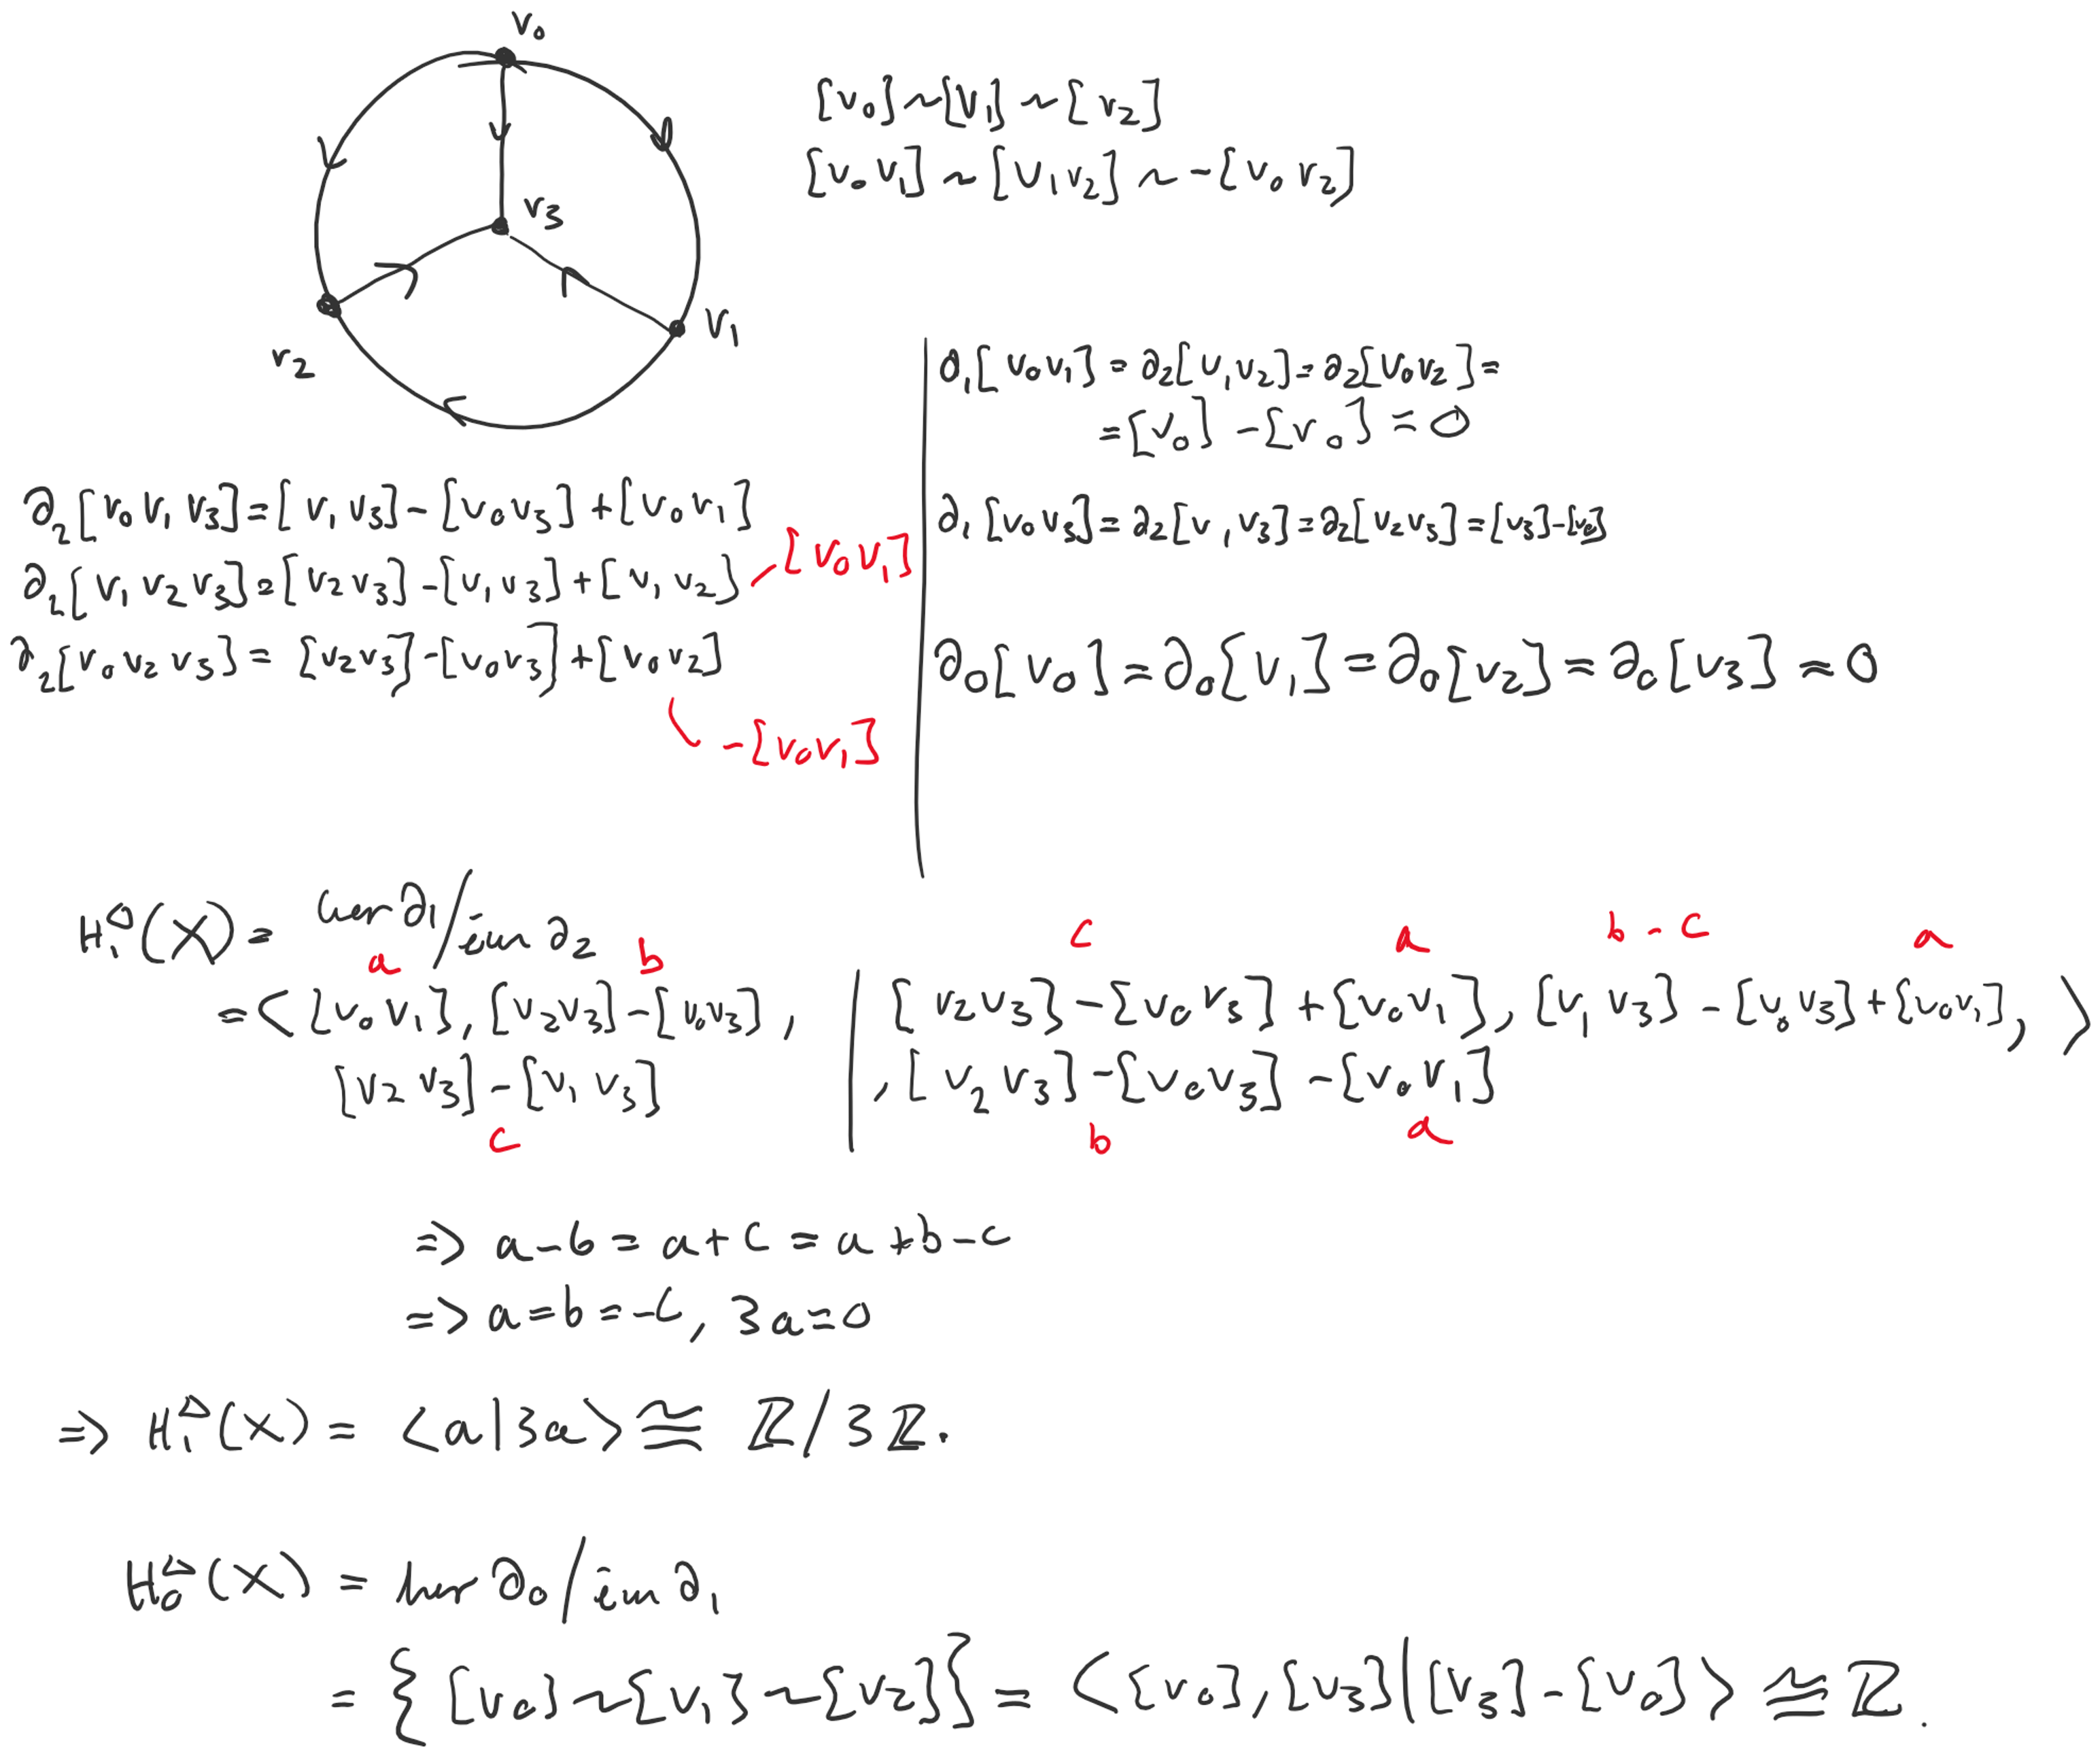
\includegraphics[width = 0.9\textwidth]{assignment2.png}
\end{center}

Noting that $\partial_2$ is injective which means $H_2(X)$ is trivial, we summarize:

\begin{itemize}
  \item $H_n^\Delta(X) = 0$ for $n \geq 3$.
  \item $H_2^\Delta(X) = 0$.
  \item $H_1^\Delta(X) = \mathbb{Z} / 3\mathbb{Z}$.
  \item $H_0^\Delta(X) = \mathbb{Z}$.
\end{itemize}



\end{proof}

\newpage

\begin{problem}
\textbf{(W)} For a finitely generated abelian group $A$, the \emph{rank} of $A$ is the maximal rank of a free abelian subgroup of $A$.
\begin{enumerate}[font=\normalfont,label=\textbf{(\alph*)}]
  \item Suppose we have a short exact sequence of abelian groups
  \[
0 \to A \overset{i}{\to} B \overset{q}{\to} C \to 0
  \]
  (this means that $i$ is injective, $q$ is surjective, and $\Im(i) = \Ker(q)$). Prove that $\Rank(B) = \Rank(A) + \Rank(C)$.

  \item Prove that the Euler characteristic of a finite $\Delta$-complex $X$ equals
  \[
\sum_{i=0}^\infty (-1)^i\Rank(H_i^\Delta (X)).
  \]
  Hint: Observe that there exist short exact sequences
  \[
0 \to \Im(\partial_{n+1}) \overset{i}{\to} \Ker(\partial_n) \overset{q}{\to} H_n(X) \to 0
  \]
  and
  \[
0 \to \Ker(\partial_n) \overset{i}{\to} C_n^\Delta (X) \overset{q}{\to} \Im(\partial_n) \to 0.
  \]
\end{enumerate}
\end{problem}

\begin{proof}[Solution]

\hfill


\begin{enumerate}[font=\normalfont,label=\textbf{(\alph*)}, wide]
  \item Let $F_A$ be a maximal free subgroup of $A$, generated by $\{f_\alpha \mid \alpha \in \mathcal{A}\}$, for some index set $\mathcal{A}$. By injectivity of $i$, each of these basis elements $f_\alpha$ are mapped to distinct elements $i(f_\alpha)$. Since $A, B, C$ are abelian, each word $\sum_{\alpha \in \mathcal{A}} f_\alpha^{k_\alpha} \in F_A$ is mapped to
  \[
i \left(\sum_{\alpha \in \mathcal{A}} f_\alpha^{k_\alpha} \right) = \sum_{\alpha \in \mathcal{A}}i \left(f_\alpha\right)^{k_\alpha},
  \]
so $\Im_i(F_A)$ is a free abelian subgroup of $B$ generated by $\{i(f_\alpha) \mid \alpha \in \mathcal{A}\}$ with rank equal to $F_A$. By exactness, $\Im(i) = \Ker(q)$ so $\Im(F_A) < \Ker(q)$. The First Isomorphism Theorem implies that $B/\Ker(q) \cong \Im(q) \iff B/\Im(i) \cong \Im(q) = C$, since $q$ is surjective. Take a maximal free subgroup $F_C < C$. Then this is also a maximal free subgroup $F_C'$ of $B/\Im(i)$, which extends to a free subgroup of $B$ by forming the subgroup consisting of words formed by one representative per basis element of $F_C'$ from the preimage of the quotient homomorphism. By abuse of notation, let this group also be denoted by $F_C'$.

Now, the group $F_B$ generated by the generators of $\Im(F_A)$ together with the generators of $F_C'$ is a free subgroup of $B$ of rank $R = \Rank(A) + \Rank(C)$, since $\Rank(\Im(F_A)) = \Rank(F_A) = \Rank(A)$, $\Rank(F_C') = \Rank(F_C) = \Rank(C)$ and $F_C'$ and $\Im(F_A)$ are mutually disjoint. The restriction of $F_B$ to $\Ker(q) = \Im(i)$ is isomorphic to $F_A$ and the quotient of $F_B$ by $\Ker(q)$ is isomorphic to $F_C$. The claim is that this group is maximally free in $B$; suppose on the contrary that there is some free group $F_B' < B$ of higher rank than $F_B$. Since $B/\Ker(q) \cong C$ and $F_C$ is maximally free in $C$, we cannot have that the image of $F_B'$ under the quotient homomorphism by $\Ker(q)$ has higher rank than $F_C$. Hence, the only possibility is that the restriction of $F_B'$ to $\Ker(q)$ has higher rank than $F_A$, but this is also impossible since $F_A$ is maximally free in $A$. Hence $F_B$ is maximally free in $B$ with rank $R = \Rank(A) + \Rank(C)$, and so $ \Rank(B) = \Rank(A) + \Rank(C)$, as desired.


\item Recall that the Euler characteristic is
\[
\chi(X) = \sum_n (-1)^nc_n,
\]
where $c_n$ is the number of $n$-cells (which in our case will be $n$-simplices) of $X$. By definition, $c_n$ is equal to $\Rank(C_n^\Delta(X))$.

The existence of a short exact sequence
\[
0 \to \Im(\partial_{n+1}) \overset{i}{\to} \Ker(\partial_n) \overset{q}{\to} H_n(X) \to 0.
\]
follows from the fact that $\Ker(\partial_n)/\Im(\partial_{n+1}) \cong H_n(X)$ by definition. Moreover, certainly $C_n^\Delta (X)/\Ker(\partial_n) \cong \Im(\partial_n)$ by the first isomorphism theorem since $\partial_n$ is a homomorphism, which implies the existence of a short exact sequence
\[
0 \to \Ker(\partial_n) \overset{i}{\to} C_n^\Delta (X) \overset{q}{\to} \Im(\partial_n) \to 0.
\]
By part \textbf{(a)}, we have that
\[
\Rank(C_n^\Delta(X))  = \Rank(\Ker(\partial_{n})) + \Rank(\Im(\partial_n))
\]
 while
 \[
 \Rank(\Ker(\partial_n))  = \Rank(\Im(\partial_{n+1})) + \Rank(H_n(X)),
\]
so
\[
\Rank(C_n^\Delta(X))  = \Rank(\Im(\partial_{n+1})) + \Rank(H_n(X)) + \Rank(\Im(\partial_n)).
\]

Plugging into the formula for the Euler characteristic we find
\[
\begin{aligned}
\chi(X) &= \sum_n (-1)^nc_n = \sum_{n = 0}^\infty (-1)^n \Rank(C_n^\Delta(X)) \\
        &= \sum_{n = 0}^\infty (-1)^n \left[ \Rank(\Im(\partial_{n+1})) + \Rank(H_n(X)) + \Rank(\Im(\partial_n)) \right] \\
        &= \sum_{n = 0}^\infty (-1)^n  \Rank(H_n(X)) + \sum_{n = 0}^\infty (-1)^n \Rank(\Im(\partial_{n+1})) + \sum_{n = 0}^\infty (-1)^n \Rank(\Im(\partial_n)) \\
        &= \Rank(\Im(\partial_0)) + \sum_{n = 0}^\infty (-1)^n  \Rank(H_n(X)) +  \sum_{n = 1}^\infty (-1)^n\left[ -\Rank(\Im(\partial_{n}))  + \Rank(\Im(\partial_{n}))\right] \\
        &= \{\text{By finiteness, the second sum is 0}\} \\
        &= \Rank(\Im(\partial_0)) + \sum_{n = 0}^\infty (-1)^n  \Rank(H_n(X)) \\
        &= \sum_{n = 0}^\infty (-1)^n  \Rank(H_n(X)), \\
\end{aligned}
\]
since the image of $\partial_0$ is the trivial group.
\end{enumerate}
\end{proof}
\end{document}
